\section{Face validation}
The problem of face validation in our context is represented by determining whether the face detected in an image belongs to a live subject or it is on a printed photo, replayed video or 3D mask. Various methods to combat such attacks have been studied and they include: face motion analysis \cite{BharadwajDVS13},\cite{PanSWL07},\cite{TirunagariPWISH15} like eye blink, lip or head movement that is effective in combating printed photos attack, face 3D shape or depth analysis \cite{MarsicoNRD12}, \cite{LagorioTCFS13} which is useful in combating 2D attacks but may require additional device, face texture analysis \cite{MaattaHP11} which have computationally low costs and are fast but might encounter difficulties in generalizability. Our implementation of the face spoof detector is based on the work of Maatta et al. presented in \cite{MaattaHP11} where the proposed approached is based on the analysis of face texture using multi-scale local binary patterns (MLBP).
\subsection{Basic Local Binary Patterns}
The LBP is a type of visual descriptor used for texture identification and classification. Firstly presented by Ojala and Harwood in 1996 in \cite{ojala1996comparative}, it is a particular case of the Texture Unit model described in 1990 in \cite{HeWang90}. The idea proposed by He\&Wang in \cite{HeWang90} was to compute the local texture for each pixel in an image based on a surrounding neighborhood of $3\times3$ pixels. The way to compute it was to compare the intensity of the central pixel $V_c$ with the intensity of each of the 8 neighbour pixels $V_{i=\overline{1,8}}$so resulting a corresponding texture unit TU with 8 elements calculated as this:
\begin{align}
	E_i = \begin{cases}
	0, & if\ V_c > V_i \\
	1, & if\ V_c = V_i \\
	2, & if\ V_c < V_i
	\end{cases}
\end{align}
The texture unit representation is then seen as a number in base 3 and transform in decimal base obtaining this way a number describing the local texture of a pixel.
A visual representation can be seen in figure 2.4
\begin{figure}[h]
	\begin{center}
		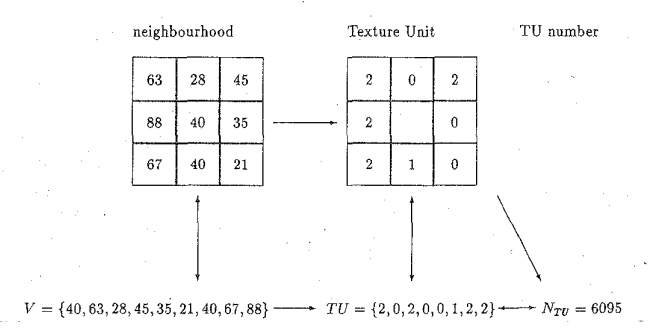
\includegraphics[width=15cm]{texture-unit-transform}
	\end{center}
	\caption[Visual representation of texture unit transform]{How \cite{HeWang90} presented the transformation of a pixel neighbourhood into a texture unit and a texture unit number}
\end{figure}

The reason why LBP is considered to be a particular case of texture unit is that the only difference from it is the function of computing the $E_i$ which differs from the one proposed by He\&Wang in that the equality case is comprised in one of the inequalities and therefore only two values, 0 and 1, are required
\begin{align}
E_i = \begin{cases}
0, & if\ V_c > V_i \\
1, & if\ V_c \leq V_i \\
\end{cases}
\end{align}
which means that the texture unit will contain 8 base 2 values

\begin{figure}[h]
	\begin{center}
		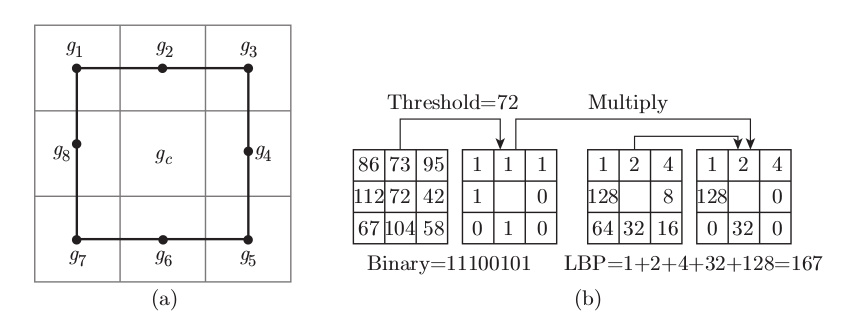
\includegraphics[width=15cm]{visual-lbp}
	\end{center}
	\caption[Visual representation of \textbf{LBP} computation]{An intuitive graphical representation of obtaining the LBP number from a $3\times3$ pixel cell presented in \cite{lu2014divided}}
\end{figure}

\subsection{Variations of the LBP}
In 2002, Ojala et al. described in \cite{OjalaPM02} an extension of the LBP from the square of $3\times3$ pixels to any size neighbourhood by considering a circle around the central pixel and sampling it's neighbours on this circle. This adds two parameters to the LBP, one being the radius $R$ of the circle and the second one being the number of sampled points $P$ on the circle.  With this new definition, we can formulate the LBP operator as being
\begin{align}
	LBP_{R,P} = \sum_{0}^{P-1}E_p*2^p
\end{align}

\begin{figure}[h]
	\begin{center}
		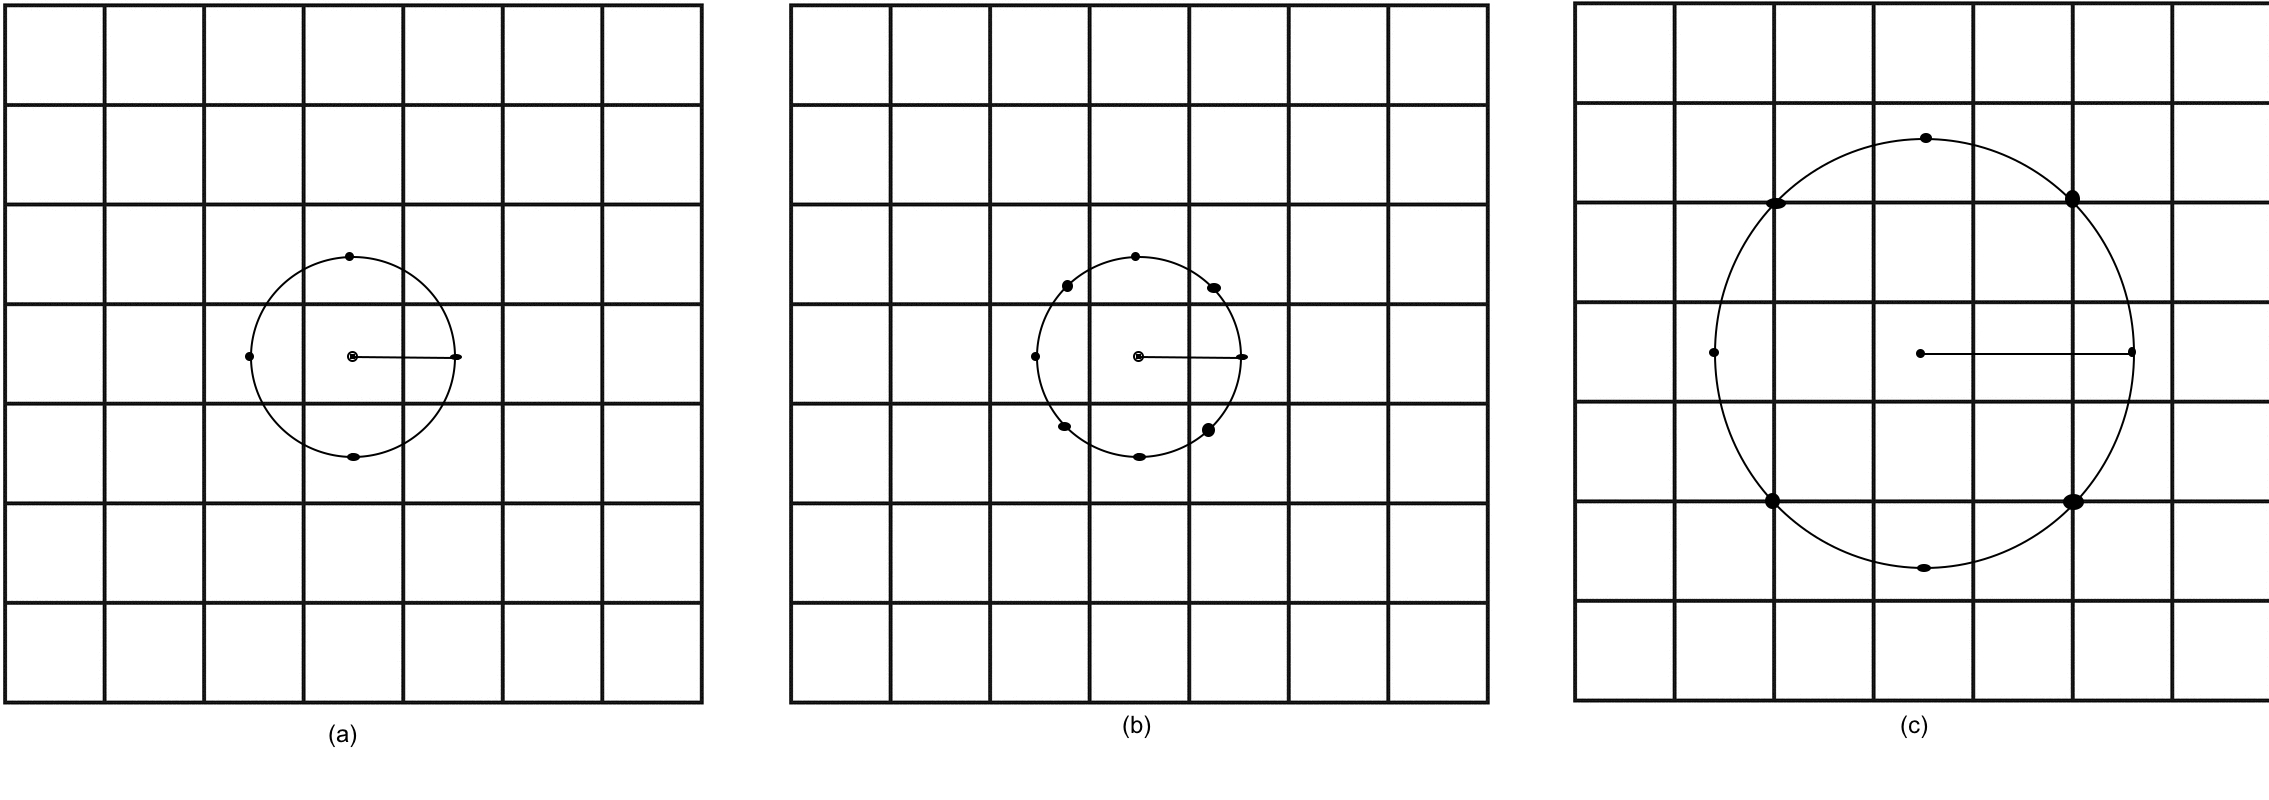
\includegraphics[width=15cm]{lbps-different-radius-sample}
	\end{center}
	\caption[Enhanced LBP visualisation]{Here we visualize the enhaced version of LBP presented in \cite{OjalaPM02}. (a) LBP with R = 1 and P = 4. (b) LBP with R = 1 and P = 8. (c) LBP with R = 2 and P = 8}
\end{figure}
As can be observed the $LBP_{R,P}$ operator produces $2^P$ values corresponding to the $2^P$ possible patterns in the texture unit TU. As the P grows linearly, the number of produces values grows exponentially therefore it is obvious that it can create computational problems for values of P not too big.

